\documentclass[]{article}
\usepackage{lmodern}
\usepackage{amssymb,amsmath}
\usepackage{ifxetex,ifluatex}
\usepackage{fixltx2e} % provides \textsubscript
\ifnum 0\ifxetex 1\fi\ifluatex 1\fi=0 % if pdftex
  \usepackage[T1]{fontenc}
  \usepackage[utf8]{inputenc}
\else % if luatex or xelatex
  \ifxetex
    \usepackage{mathspec}
  \else
    \usepackage{fontspec}
  \fi
  \defaultfontfeatures{Ligatures=TeX,Scale=MatchLowercase}
\fi
% use upquote if available, for straight quotes in verbatim environments
\IfFileExists{upquote.sty}{\usepackage{upquote}}{}
% use microtype if available
\IfFileExists{microtype.sty}{%
\usepackage{microtype}
\UseMicrotypeSet[protrusion]{basicmath} % disable protrusion for tt fonts
}{}
\usepackage[margin=1in]{geometry}
\usepackage{hyperref}
\hypersetup{unicode=true,
            pdfborder={0 0 0},
            breaklinks=true}
\urlstyle{same}  % don't use monospace font for urls
\usepackage{graphicx,grffile}
\makeatletter
\def\maxwidth{\ifdim\Gin@nat@width>\linewidth\linewidth\else\Gin@nat@width\fi}
\def\maxheight{\ifdim\Gin@nat@height>\textheight\textheight\else\Gin@nat@height\fi}
\makeatother
% Scale images if necessary, so that they will not overflow the page
% margins by default, and it is still possible to overwrite the defaults
% using explicit options in \includegraphics[width, height, ...]{}
\setkeys{Gin}{width=\maxwidth,height=\maxheight,keepaspectratio}
\IfFileExists{parskip.sty}{%
\usepackage{parskip}
}{% else
\setlength{\parindent}{0pt}
\setlength{\parskip}{6pt plus 2pt minus 1pt}
}
\setlength{\emergencystretch}{3em}  % prevent overfull lines
\providecommand{\tightlist}{%
  \setlength{\itemsep}{0pt}\setlength{\parskip}{0pt}}
\setcounter{secnumdepth}{0}
% Redefines (sub)paragraphs to behave more like sections
\ifx\paragraph\undefined\else
\let\oldparagraph\paragraph
\renewcommand{\paragraph}[1]{\oldparagraph{#1}\mbox{}}
\fi
\ifx\subparagraph\undefined\else
\let\oldsubparagraph\subparagraph
\renewcommand{\subparagraph}[1]{\oldsubparagraph{#1}\mbox{}}
\fi

%%% Use protect on footnotes to avoid problems with footnotes in titles
\let\rmarkdownfootnote\footnote%
\def\footnote{\protect\rmarkdownfootnote}

%%% Change title format to be more compact
\usepackage{titling}

% Create subtitle command for use in maketitle
\newcommand{\subtitle}[1]{
  \posttitle{
    \begin{center}\large#1\end{center}
    }
}

\setlength{\droptitle}{-2em}

  \title{}
    \pretitle{\vspace{\droptitle}}
  \posttitle{}
    \author{}
    \preauthor{}\postauthor{}
    \date{}
    \predate{}\postdate{}
  

\begin{document}

\section{Boltzmann machine}\label{boltzmann-machine}

\begin{figure}
\centering
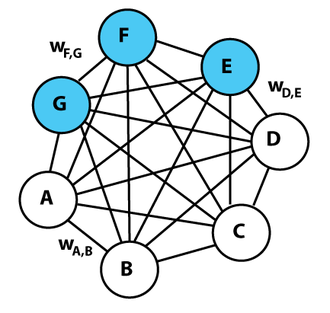
\includegraphics{data/220px-Boltzmannexamplev1.png}
\caption{Boltzmann machine}
\end{figure}

Can be considered as a computational neuroscience dream. Can a network
learn by itself?

Boltzmann machine is fully connected: all visible and hidden units
connected to each other. This implies there is no structure imposed on
the network. Analogous to the human nervous system where the sensory
neurons are the visible units and other neurons are hidden units.
Equilibrium state is attained by minimizing the energy:

\[E = -\big(\sum_{i<j}w_{ij}s_is_j + \sum_{i}b_is_i\big)\]

Boltzmann machines are very difficult to train in practice.

\section{Restricted Boltzmann
machine}\label{restricted-boltzmann-machine}

Connections are restricted between visible and hidden units.
Visible-visible and hidden-hidden connections are absent.

\[E(v, h) = -\big(\sum_{i=1}^{D}\sum_{j=1}^{M}w_{ij}v_ih_j + \sum_{i=1}^{D}b_iv_i + \sum_{j=1}^{M}c_jh_j\big) = -(v^Twh + b^Tv + c^Th)\]

\[p(v,h) \propto e^{-E(v,h)}\]

\[p(v,h) = \frac{1}{Z}e^{-E(v,h)}, Z = \sum_v\sum_he^{-E(v,h)}; \sum_v\sum_hp(v,h)=1\]

Z is the partition function.

This comes from
\(p_i \propto e^{-E_i/(kT)}; p_i = \frac{1}{Z} e^{-E_i/(kT)}; Z = \sum_ie^{-E_i/(kT)}\)

\subsection{Intractability}\label{intractability}

Calculating the sum for all possible states is computationally
expensive.

If v has length D and h has length M, there are
\(2^D \times 2^M = 2^{D+M}\) possibilities. MNIST example: D = 784, M =
100.

\subsection{Training}\label{training}

For simplicity let us assume that both visible and hidden units are
binary encoded. Eg:
\(v_i = \begin{cases}0&x_i/255\le0.5\\1&x_i/255>0.5\end{cases}\)

\subsubsection{Probabilities}\label{probabilities}

\[p(v|h) = p(v,h)/p(h);p(h|v) = p(v,h)/p(v)\]

\textbf{Marginals} \(p(v) = \sum_hp(v,h); p(h) = \sum_vp(v,h)\)

\[p(v,h) = \frac{1}{Z}exp(v^Twh+b^Tv+c^th)\]

\[p(v) = \sum_h\frac{1}{Z}exp(v^Twh+b^Tv+c^th)\]

\[\implies p(h|v) = \frac{exp(v^Twh+b^Tv+c^th)}{\sum_h\exp(v^Twh+b^Tv+c^th)} = \frac{1}{Z'}exp(v^Twh+b^Tv+c^th)\]

Sum over h makes this intractable.

\[\implies p(h|v) = \frac{1}{Z'}exp(\sum_{i=1}^{D}\sum_{j=1}^{M}w_{ij}v_ih_j + \sum_{i=1}^{D}b_iv_i + \sum_{j=1}^Dc_jh_j)\]
\[= \frac{1}{Z'}exp(\sum_{i=1}^{D}b_iv_i)\prod_{j=1}^Mexp(\sum_{i=1}^Dw_{ij}v_ih_j+c_jh_j) = \frac{1}{Z''}\prod_{j=1}^Mexp(\sum_{i=1}^Dw_{ij}v_ih_j+c_jh_j)\]

The last step was possible because v is conditioned on.

\[\implies p(h|v) = \frac{1}{Z''}\prod_{j=1}^Mexp(\sum_{i=1}^Dh_j\{w_{ij}v_i+c_j\})\]

Hidden units are independent
\(p(h_j|v) = \frac{1}{Z'''}exp(h_j\sum_{i=1}^D\{w_{ij}v_i+c_j\})\)
because they are not connected to each other.

Since \(h_j\) is binary,
\(p(h_j=1|v) = \frac{1}{Z'''}exp(\sum_{i=1}^D\{w_{ij}v_i+c_j\}), p(h_j=0|v)=\frac{1}{Z'''} \implies Z'''= 1 + exp(\sum_{i=1}^D\{w_{ij}v_i+c_j\}); p(h_j=1|v) = sigmoid(\sum_{i=1}^Dw_{ij}v_i+c_j) = sigmoid(w^Tv + c)\).
This gives a vector of probabilities. Similar derivation can be used for
\(p(v=1|h)\)


\end{document}
